\documentclass[12pt,]{krantz}
\usepackage{lmodern}
\usepackage{amssymb,amsmath}
\usepackage{ifxetex,ifluatex}
\usepackage{fixltx2e} % provides \textsubscript
\ifnum 0\ifxetex 1\fi\ifluatex 1\fi=0 % if pdftex
  \usepackage[T1]{fontenc}
  \usepackage[utf8]{inputenc}
\else % if luatex or xelatex
  \ifxetex
    \usepackage{mathspec}
  \else
    \usepackage{fontspec}
  \fi
  \defaultfontfeatures{Ligatures=TeX,Scale=MatchLowercase}
    \setmonofont[Mapping=tex-ansi,Scale=0.7]{Source Code Pro}
\fi
% use upquote if available, for straight quotes in verbatim environments
\IfFileExists{upquote.sty}{\usepackage{upquote}}{}
% use microtype if available
\IfFileExists{microtype.sty}{%
\usepackage{microtype}
\UseMicrotypeSet[protrusion]{basicmath} % disable protrusion for tt fonts
}{}
\usepackage[unicode=true]{hyperref}
\PassOptionsToPackage{usenames,dvipsnames}{color} % color is loaded by hyperref
\hypersetup{
            pdftitle={Introduction to Data Science},
            pdfauthor={Hui Lin and Ming Li},
            colorlinks=true,
            linkcolor=Maroon,
            citecolor=Blue,
            urlcolor=Blue,
            breaklinks=true}
\urlstyle{same}  % don't use monospace font for urls
\usepackage{natbib}
\bibliographystyle{apalike}
\usepackage{longtable,booktabs}
\usepackage{graphicx,grffile}
\makeatletter
\def\maxwidth{\ifdim\Gin@nat@width>\linewidth\linewidth\else\Gin@nat@width\fi}
\def\maxheight{\ifdim\Gin@nat@height>\textheight\textheight\else\Gin@nat@height\fi}
\makeatother
% Scale images if necessary, so that they will not overflow the page
% margins by default, and it is still possible to overwrite the defaults
% using explicit options in \includegraphics[width, height, ...]{}
\setkeys{Gin}{width=\maxwidth,height=\maxheight,keepaspectratio}
\IfFileExists{parskip.sty}{%
\usepackage{parskip}
}{% else
\setlength{\parindent}{0pt}
\setlength{\parskip}{6pt plus 2pt minus 1pt}
}
\setlength{\emergencystretch}{3em}  % prevent overfull lines
\providecommand{\tightlist}{%
  \setlength{\itemsep}{0pt}\setlength{\parskip}{0pt}}
\setcounter{secnumdepth}{5}
% Redefines (sub)paragraphs to behave more like sections
\ifx\paragraph\undefined\else
\let\oldparagraph\paragraph
\renewcommand{\paragraph}[1]{\oldparagraph{#1}\mbox{}}
\fi
\ifx\subparagraph\undefined\else
\let\oldsubparagraph\subparagraph
\renewcommand{\subparagraph}[1]{\oldsubparagraph{#1}\mbox{}}
\fi
\usepackage{booktabs}
\usepackage{longtable}
\usepackage[bf,singlelinecheck=off]{caption}

\setmainfont[UprightFeatures={SmallCapsFont=AlegreyaSC-Regular}]{Alegreya}

\usepackage{framed,color}
\definecolor{shadecolor}{RGB}{248,248,248}

\renewcommand{\textfraction}{0.05}
\renewcommand{\topfraction}{0.8}
\renewcommand{\bottomfraction}{0.8}
\renewcommand{\floatpagefraction}{0.75}

\renewenvironment{quote}{\begin{VF}}{\end{VF}}
\let\oldhref\href
\renewcommand{\href}[2]{#2\footnote{\url{#1}}}

\ifxetex
  \usepackage{letltxmacro}
  \setlength{\XeTeXLinkMargin}{1pt}
  \LetLtxMacro\SavedIncludeGraphics\includegraphics
  \def\includegraphics#1#{% #1 catches optional stuff (star/opt. arg.)
    \IncludeGraphicsAux{#1}%
  }%
  \newcommand*{\IncludeGraphicsAux}[2]{%
    \XeTeXLinkBox{%
      \SavedIncludeGraphics#1{#2}%
    }%
  }%
\fi

\makeatletter
\newenvironment{kframe}{%
\medskip{}
\setlength{\fboxsep}{.8em}
 \def\at@end@of@kframe{}%
 \ifinner\ifhmode%
  \def\at@end@of@kframe{\end{minipage}}%
  \begin{minipage}{\columnwidth}%
 \fi\fi%
 \def\FrameCommand##1{\hskip\@totalleftmargin \hskip-\fboxsep
 \colorbox{shadecolor}{##1}\hskip-\fboxsep
     % There is no \\@totalrightmargin, so:
     \hskip-\linewidth \hskip-\@totalleftmargin \hskip\columnwidth}%
 \MakeFramed {\advance\hsize-\width
   \@totalleftmargin\z@ \linewidth\hsize
   \@setminipage}}%
 {\par\unskip\endMakeFramed%
 \at@end@of@kframe}
\makeatother

% \renewenvironment{Shaded}{\begin{kframe}}{\end{kframe}}

\newenvironment{rmdblock}[1]
  {
  \begin{itemize}
  \renewcommand{\labelitemi}{
    \raisebox{-.7\height}[0pt][0pt]{
      {\setkeys{Gin}{width=3em,keepaspectratio}\includegraphics{images/#1}}
    }
  }
  \setlength{\fboxsep}{1em}
  \begin{kframe}
  \item
  }
  {
  \end{kframe}
  \end{itemize}
  }
\newenvironment{rmdnote}
  {\begin{rmdblock}{note}}
  {\end{rmdblock}}
\newenvironment{rmdcaution}
  {\begin{rmdblock}{caution}}
  {\end{rmdblock}}
\newenvironment{rmdimportant}
  {\begin{rmdblock}{important}}
  {\end{rmdblock}}
\newenvironment{rmdtip}
  {\begin{rmdblock}{tip}}
  {\end{rmdblock}}
\newenvironment{rmdwarning}
  {\begin{rmdblock}{warning}}
  {\end{rmdblock}}

\usepackage{makeidx}
\makeindex

\urlstyle{tt}

\usepackage{amsthm}
\makeatletter
\def\thm@space@setup{%
  \thm@preskip=8pt plus 2pt minus 4pt
  \thm@postskip=\thm@preskip
}
\makeatother

\frontmatter

\title{Introduction to Data Science}
\author{Hui Lin and Ming Li}
\date{2017-12-10}

\usepackage{amsthm}
\newtheorem{theorem}{Theorem}[chapter]
\newtheorem{lemma}{Lemma}[chapter]
\theoremstyle{definition}
\newtheorem{definition}{Definition}[chapter]
\newtheorem{corollary}{Corollary}[chapter]
\newtheorem{proposition}{Proposition}[chapter]
\theoremstyle{definition}
\newtheorem{example}{Example}[chapter]
\theoremstyle{remark}
\newtheorem*{remark}{Remark}
\begin{document}
\maketitle

%\cleardoublepage\newpage\thispagestyle{empty}\null
%\cleardoublepage\newpage\thispagestyle{empty}\null
%\cleardoublepage\newpage
\thispagestyle{empty}
\begin{center}
%\includegraphics{images/dedication.pdf}
\end{center}

\setlength{\abovedisplayskip}{-5pt}
\setlength{\abovedisplayshortskip}{-5pt}

{
\hypersetup{linkcolor=black}
\setcounter{tocdepth}{2}
\tableofcontents
}
\listoftables
\listoffigures
\chapter*{Preface}\label{preface}


During the first couple years of our career as data scientists, we were
bewildered by all kinds of data science hype. There is a lack of
definition of many basic terminologies such as ``Big Data'' and ``Data
Science.'' How big is big? If someone ran into you asked what data
science was all about, what would you tell them? What is the difference
between the sexy role ``Data Scientist'' and the traditional ``Data
Analyst''? How suddenly came all kinds of machine algorithms? All those
struck us as confusing and vague as real-world data scientists! But we
always felt that there was something real there. After applying data
science for many years, we explored it more and had a much better idea
about data science. And this book is our endeavor to make data science
to a more legitimate field.

\section*{Goal of the Book}\label{goal-of-the-book}


This is an introductory book to data science with a specific focus on
the application. Data Science is a cross-disciplinary subject involving
hands-on experience and business problem-solving exposures. The majority
of existing introduction books on data science are about the modeling
techniques and the implementation of models using R or Python. However,
they fail to introduce data science in a context of the industrial
environment. Moreover, a crucial part, the art of data science in
practice, is often missing. This book intends to fill the gap.

Some key features of this book are as follows:

\begin{itemize}
\item
  It is comprehensive. It covers not only technical skills but also soft
  skills and big data environment in the industry.
\item
  It is hands-on. We provide the data and repeatable R and Python code.
  You can repeat the analysis in the book using the data and code
  provided. We also suggest you perform the analyses with your data
  whenever possible. You can only learn data science by doing it!
\item
  It is based on context. We put methods in the context of industrial
  data science questions.
\item
  Where appropriate, we point you to more advanced materials on models
  to dive deeper
\end{itemize}

\section*{Who This Book Is For}\label{who-this-book-is-for}


Non-mathematical readers will appreciate the emphasis on problem-solving
with real data across a wide variety of applications and the
reproducibility of the companion R and python code.

Readers should know basic statistical ideas, such as correlation and
linear regression analysis. While the text is biased against complex
equations, a mathematical background is needed for advanced topics.

\section*{What This Book Covers}\label{what-this-book-covers}


Based on industry experience, this book outlines the real world scenario
and points out pitfalls data science practitioners should avoid. It also
covers big data cloud platform and the art of data science such as soft
skills. We use R as the main tool and provide code for both R and
Python.

\section*{Conventions}\label{conventions}


\section*{Acknowledgements}\label{acknowledgements}


\mainmatter

\chapter{Introduction}\label{introduction}

Interest in data science is at an all-time high and has exploded in
popularity in the last couple of years. Data scientists today are from
various backgrounds. If someone ran into you asked what data science was
all about, what would you tell them? It is not easy to answer. Data
science is one of the areas where you ask ten people who will give ten
different answers. It is not well-defined as an academic subject but
broadly used in the industry. Media has been hyping about ``Data
Science'' ``Big Data'' and ``Artificial Intelligence'' over the fast few
years. With the data science hype picking up stream, many professionals
changed their titles to ``Data Scientist'' without any of the necessary
qualifications. Your first reaction to all of this might be some
combination of skepticism and confusion. We want to address this up
front that: we had that exact reaction. To make things clear, let's
start with the fundamental question.

\section{What is data science?}\label{what-is-data-science}

David Donoho \citep{data50} summarizes in ``50 Years of Data Science''
the main recurring ``Memes'' about data sciences:

\begin{enumerate}
\def\labelenumi{\arabic{enumi}.}
\tightlist
\item
  The `Big Data' Meme
\item
  The `Skills' Meme
\item
  The `Jobs' Meme
\end{enumerate}

Everyone should have heard about big data. Data science trainees now
need the skills to cope with such big data sets. What are those skills?
You may hear about: Hadoop, a system using Map/Reduce to process large
data sets distributed across a cluster of computers. The new skills are
for dealing with organizational artifacts of large-scale cluster
computing but not for better solving the real problem. A lot of data on
its own is worthless. It isn't the size of the data that's important.
It's what you do with it. The big data skills that so many are touting
today are not skills for better solving the real problem of inference
from data.

We are transiting to universal connectivity with a deluge of data
filling telecom servers. But these facts don't immediately create a
science. The statisticians and computer scientists have been laying the
groundwork for data science for at least 50 years. Today's data science
is an enlargement and combination of statistics and computer science
rather than a brand new discipline.

Data Science doesn't come out of the blue. Its predecessor is data
analysis. Back in 1962, John Tukey wrote in ``The Future of Data
Analysis'':

\begin{quote}
For a long time I have thought I was a statistician, interested in
inferences from the particular to the general. But as I have watched
mathematical statistics evolve, I have had cause to wonder and to doubt.
\ldots{}All in all, I have come to feel that my central interest is in
data analysis, which I take to include, among other things: procedures
for analyzing data, techniques for interpreting the results of such
procedures, ways of planning the gathering of data to make its analysis
easier, more precise or more accurate, and all the machinery and results
of (mathematical) statistics which apply to analyzing data.
\end{quote}

It deeply shocked his academic readers. Aren't you supposed to present
something mathematically precise, such as definitions, theorems, and
proofs? If we use one sentence to summarize what John said, it is:

\begin{quote}
data analysis is more than mathematics.
\end{quote}

In September 2015, the University of Michigan made plans to invest \$100
million over the next five years in a new Data Science Initiative (DSI)
that will enhance opportunities for student and faculty researchers
across the university to tap into the enormous potential of big data.
How does DSI define Data science? Their website gives us an idea:

\begin{quote}
``This coupling of scientific discovery and practice involves the
collection, management, processing, analysis, visualization, and
interpretation of vast amounts of heterogeneous data associated with a
diverse array of scientific, translational, and interdisciplinary
applications.''
\end{quote}

How about data scientist? Here is a list of somewhat whimsical
definitions for a ``data scientist'':

\begin{itemize}
\tightlist
\item
  ``A data scientist is a data analyst who lives in California''
\item
  ``A data scientist is someone who is better at statistics than any
  software engineer and better at software engineering than any
  statistician.''
\item
  ``A data scientist is a statistician who lives in San Francisco.''
\item
  ``Data Science is statistics on a Mac.''
\end{itemize}

There is lots of confusion between Data Scientist, Statistician,
Business/Financial/Risk(etc.) Analyst and BI professional due to the
apparent intersections among skillsets. We see data science as a
discipline to make sense of data. The techniques and methodologies of
data science stem from the fields of computer science and statistics.
One of the most well-cited diagrams describing the area comes from Drew
Conway where he suggested data science is the intersection of hacking
skills, math and stats knowledge, and substantial expertise. This
diagram might be a bit of an oversimplification, but it's a great start.

In the obscenity case of Jacobellis v. Ohio (1964), Potter Stewart wrote
in his short concurrence that ``hard-core pornography'' was hard to
define, but that ``I know it when I see it.'' This applies to many
things including data science. It is hard to define, but you know it
when you see it.

So instead of figuring out a good definition, we are going to sketch the
history of data science, show you what kind of questions data science
can answer, and describe the skills required for being a data scientist.
We hope this can give you a better depiction of data science.

\begin{figure}[htbp]
\centering
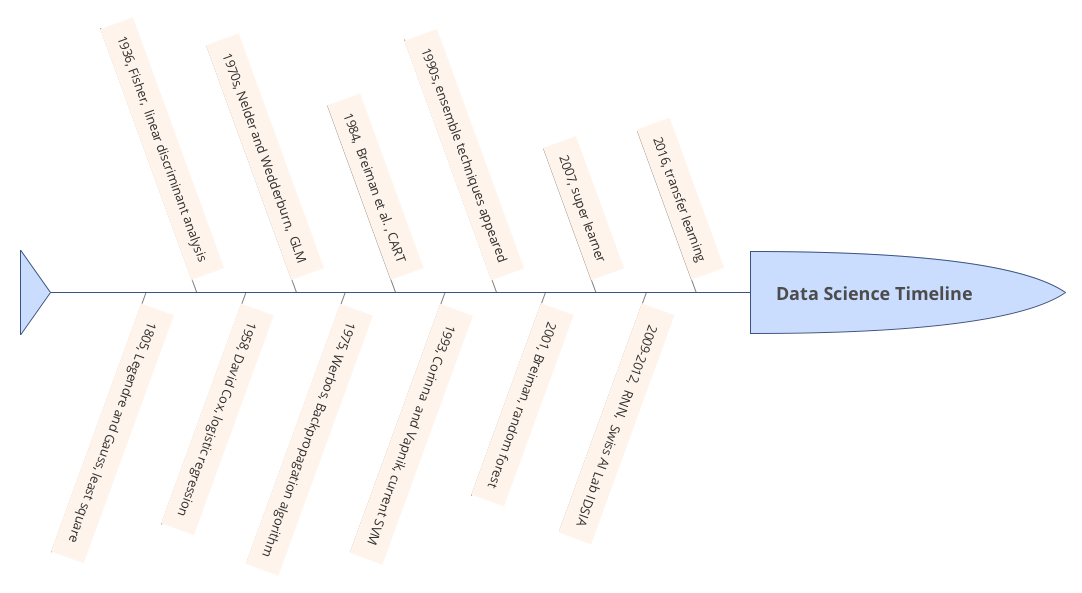
\includegraphics{images/DataScienceTimeline.png}
\caption{Data Science Timeline}
\end{figure}

In the early 19th century when Legendre and Gauss came up the least
squares method for linear regression, only physicists would use it to
fit linear regression. Now, even non-technical people can fit linear
regressions using excel. In 1936 Fisher came up with linear discriminant
analysis. In the 1940s, we had another widely used model -- logistic
regression. In the 1970s, Nelder and Wedderburn formulated ``generalized
linear model (GLM)'' which:

\begin{quote}
``generalized linear regression by allowing the linear model to be
related to the response variable via a link function and by allowing the
magnitude of the variance of each measurement to be a function of its
predicted value.'' {[}from Wikipedia{]}
\end{quote}

By the end of the 1970s, there was a range of analytical models and most
of them were linear because computers were not powerful enough to fit
non-linear model until the 1980s.

In 1984 Breiman et al. introduced classification and regression tree
(CART) which is one of the oldest and most utilized classifications and
regression techniques. After that Ross Quinlan came up with more tree
algorithms such as ID3, C4.5, and C5.0. In the 1990s, ensemble
techniques (methods that combine many models' predictions) began to
appear. Bagging is a general approach that uses bootstrapping in
conjunction with any regression or classification model to construct an
ensemble. Based on the ensemble idea, Breiman came up with random forest
in 2001. Later, Yoav Freund and Robert Schapire came up with the
AdaBoost.M1 algorithm. Benefiting from the increasing availability of
digitized information, and the possibility to distribute that via the
internet, the toolbox has been expanding fast. The applications include
business, health, biology, social science, politics, etc.

John Tukey identified four forces driving data analysis (there was no
``data science'' then):

\begin{enumerate}
\def\labelenumi{\arabic{enumi}.}
\tightlist
\item
  The formal theories of math and statistics
\item
  Acceleration of developments in computers and display devices
\item
  The challenge, in many fields, of more and ever larger bodies of data
\item
  The emphasis on quantification in an ever wider variety of disciplines
\end{enumerate}

Tukey's 1962 list is surprisingly modern. Let's inspect those points in
today's context. There is always a time gap between a theory and its
application. We had the theories much earlier than application.
Fortunately, for the past 50 years, statisticians have been laying the
theoretical groundwork for constructing ``data science'' today. The
development of computers enables us to calculate much faster and deliver
results in a friendly and intuitive way. The striking transition to the
internet of things generates vast amounts of commercial data. Industries
have also sensed the value of exploiting that data. Data science seems
certain to be a major preoccupation of commercial life in coming
decades. All the four forces John identified exist today and have been
driving data science.

\section{What kind of questions can data science
solve?}\label{what-kind-of-questions-can-data-science-solve}

\subsection{Prerequisites}\label{prerequisites}

Data science is not a panacea, and data scientists are not magicians.
There are problems data science can't help. It is best to make a
judgment as early in the analytical cycle as possible. Tell your clients
honestly and clearly when you figure data analytics can't give the
answer they want. What kind of questions can data science solve? What
are the requirements for our question?

\begin{enumerate}
\def\labelenumi{\arabic{enumi}.}
\tightlist
\item
  Your question needs to be specific enough
\end{enumerate}

Look at two examples:

\begin{itemize}
\tightlist
\item
  Question 1: How can I increase product sales?
\item
  Question 2: Is the new promotional tool introduced at the beginning of
  this year boosting the annual sales of P1197 in Iowa and Wisconsin?
  (P1197 is an impressive corn seed product from DuPont Pioneer)
\end{itemize}

It is easy to see the difference between the two questions. Question 1
is a grammatically correct question, but it is proper for data analysis
to answer. Why? It is too general. What is the response variable here?
Product sales? Which product? Is it annual sales or monthly sales? What
are the candidate predictors? You nearly can't get any useful
information from the questions. In contrast, question 2 is much more
specific. From the analysis point of view, the response variable is
clearly ``annual sales of P1197 in Iowa and Wisconsin''. Even we don't
know all the predictors, but the variable of interest is ``the new
promotional tool introduced early this year.'' We want to study the
impact of the promotion of the sales. You can start from there and move
on to figure out other variables need to include in the model by further
communication.

As a data scientist, you may start with something general and unspecific
like question 1 and eventually get to question 2. Effective
communication and in-depth domain knowledge about the business problem
are essential to convert a general business question into a solvable
analytical problem. Domain knowledge helps data scientist communicate
with the language the other people can understand and obtain the
required information.

However, defining the question and variables involved don't guarantee
that you can answer it. I have encountered a well-defined supply chain
problem. My client asked about the stock needed for a product in a
particular area. Why can not this question be answered? I did fit a
Multivariate Adaptive Regression Spline (MARS) model and thought I found
a reasonable solution. But it turned out later that the data they gave
me was inaccurate. In some areas, only estimates of past supply figures
were available. The lesson lends itself to the next point.

\begin{enumerate}
\def\labelenumi{\arabic{enumi}.}
\setcounter{enumi}{1}
\tightlist
\item
  You need to have sound and relevant data
\end{enumerate}

One cannot make a silk purse out of a sow's ear. Data scientists need
data, sound and relevant data. The supply problem is a case in point.
There was relevant data, but not sound. All the later analytics based on
that data was a building on sand. Of course, data nearly almost have
noise, but it has to be in a certain range. Generally speaking, the
accuracy requirement for the independent variables of interest and
response variable is higher than others. In question 2, it is data
related to the ``new promotion'' and ``sales of P1197''.

The data has to be helpful for the question. If you want to predict
which product consumers are most likely to buy in the next three months,
you need to have historical purchasing data: the last buying time, the
amount of invoice, coupons and so on. Information about customers'
credit card number, ID number, the email address is not going to help.

Often the quality of the data is more important than the quantity, but
the quantity cannot be overlooked. In the premise of guaranteeing
quality, usually the more data, the better. If you have a specific and
reasonable question, also sound and relevant data, then congratulations,
you can start playing data science!

\subsection{Problem type}\label{problem-type}

Many of the data science books classify the various models from a
technical point of view. Such as supervised vs.~unsupervised models,
linear vs.~nonlinear models, parametric models vs.~non-parametric
models, and so on. Here we will continue on ``problem-oriented'' track.
We first introduce different groups of real problems and then present
which models can be used to answer the corresponding category of
questions.

\begin{figure}[htbp]
\centering
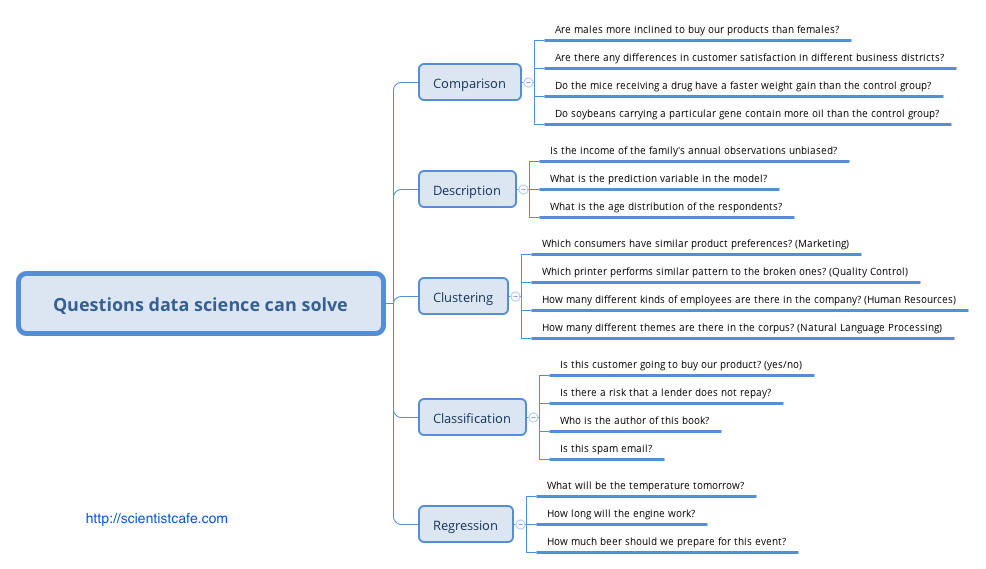
\includegraphics{images/DataScienceQuestion.png}
\caption{Data Science Questions}
\end{figure}

\begin{enumerate}
\def\labelenumi{\arabic{enumi}.}
\tightlist
\item
  Comparison
\end{enumerate}

The first common problem is to compare different groups. Such as: Is A
better in some way than B? Or more comparisons: Is there any difference
among A, B, C in a certain aspect? Here are some examples:

\begin{itemize}
\tightlist
\item
  Are the purchasing amounts different between consumers receiving
  coupons and those without coupons?
\item
  Are males more inclined to buy our products than females?
\item
  Are there any differences in customer satisfaction in different
  business districts?
\item
  Do the mice receiving a drug have a faster weight gain than the
  control group?
\item
  Do soybeans carrying a particular gene contain more oil than the
  control group?
\end{itemize}

For those problems, it is usually to start exploring from the summary
statistics and visualization by groups. After a preliminary
visualization, you can test the differences between treatment and
control group statistically. The commonly used statistical tests are
chi-square test, t-test, and ANOVA. There are also methods using
Bayesian methods. In biology industry, such as new drug development,
crop breeding, mixed effect models are the dominant technique.

\begin{enumerate}
\def\labelenumi{\arabic{enumi}.}
\setcounter{enumi}{1}
\tightlist
\item
  Description
\end{enumerate}

In the problem such as customer segmentation, after you cluster the
sample, the next step is to figure out the profile of each class by
comparing the descriptive statistics of the various variables. Questions
of this kind are:

\begin{itemize}
\tightlist
\item
  Is the income of the family's annual observations unbiased?
\item
  What is the mean/variance of the monthly sales volume of a product in
  different regions?
\item
  What is the difference in the magnitude of the variable? (Decide
  whether the data needs to be standardized)
\item
  What is the prediction variable in the model?
\item
  What is the age distribution of the respondents?
\end{itemize}

Data description is often used to check data, find the appropriate data
preprocessing method, and demonstrate the model results.

\begin{enumerate}
\def\labelenumi{\arabic{enumi}.}
\setcounter{enumi}{2}
\tightlist
\item
  Clustering
\end{enumerate}

Clustering is a widespread problem, which is usually related to
classification. Clustering answers questions like:

\begin{itemize}
\tightlist
\item
  Which consumers have similar product preferences? (Marketing)
\item
  Which printer performs similar pattern to the broken ones? (Quality
  Control)
\item
  How many different kinds of employees are there in the company? (Human
  Resources)
\item
  How many different themes are there in the corpus? (Natural Language
  Processing)
\end{itemize}

Note that clustering is unsupervised learning. The most common
clustering algorithms include K-Means and Hierarchical Clustering.

\begin{enumerate}
\def\labelenumi{\arabic{enumi}.}
\setcounter{enumi}{3}
\tightlist
\item
  Classification
\end{enumerate}

Usually, a labeled sample set is used as a training set to train the
classifier. Then the classifier is used to predict the category of a
future sample. Here are some example questions:

\begin{itemize}
\tightlist
\item
  Is this customer going to buy our product? (yes/no)
\item
  Is there a risk that a lender does not repay?
\item
  Who is the author of this book?
\item
  Is this spam email?
\end{itemize}

There are hundreds of classifiers. In practice, we do not have to try
all the models as long as we fit in several of the best models in most
cases.

\begin{enumerate}
\def\labelenumi{\arabic{enumi}.}
\setcounter{enumi}{4}
\tightlist
\item
  Regression
\end{enumerate}

In general, regression deals with the problem of ``how much is it?'' and
return a numerical answer. In some cases, it is necessary to coerce the
model results to be 0, or round the result to the nearest integer. It is
the most common problem.

\begin{itemize}
\tightlist
\item
  What will be the temperature tomorrow?
\item
  What will be the company's sales in the fourth quarter of this year?
\item
  How long will the engine work?
\item
  How much beer should we prepare for this event?
\end{itemize}

\section{What are the required skills for a data
scientist?}\label{what-are-the-required-skills-for-a-data-scientist}

We talked about the bewildering definitions of data scientist. What are
the required skills for a data scientist?

\begin{itemize}
\tightlist
\item
  Educational Background
\end{itemize}

Most of the data scientists today have undergraduate or higher degree
from one of the following areas: computer science, electronic
engineering, mathematics or statistics. According to a 2017 survey, 25\%
of US data scientists have a Ph.D.~degree, 64\% have a Master's degree,
and 11\% are Bachelors.

\begin{itemize}
\tightlist
\item
  Database Skills
\end{itemize}

Data scientists in the industry need to use SQL to pull data from the
database. So it is necessary to be familiar with how data is structured
and how to do basic data manipulation using SQL. Many
statistics/mathematics students do not have experience with SQL in
school. Don't worry. If you are proficient in one programming language,
it is easy to pick up SQL. The main purpose of graduate school should be
to develop the ability to learn and analytical thinking rather than the
technical skills. Even the technical skills are necessary to enter the
professional area. Most of the skills needed at work are not taught in
school.

\begin{itemize}
\tightlist
\item
  Programming Skills
\end{itemize}

Programming skills are critical for data scientists. According to a 2017
survey from
\href{http://www.burtchworks.com/2017/06/19/2017-sas-r-python-flash-survey-results/}{Burtch
Works}, 97\% of the data scientists today using R or Python. We will
focus on R in this book, but both are great tools for data science.
There is not one ``have-to-use'' tool. The goal is to solve the problem
not which tool to choose. However, a good tool needs to be flexible and
scalable.

\begin{itemize}
\tightlist
\item
  Modeling Skills
\end{itemize}

Data scientists need to know statistical and machine learning models.
There is no clear line separating these two. Many statistical models are
also machine learning models, vice versa. Generally speaking, a data
scientist is familiar with basic statistical tests such as t-test,
chi-square test, and analysis of variance. They can explain the
difference between Spearman rank correlation and Pearson correlation, be
aware of basic sampling schemes, such as Simple Random Sampling,
Stratified Random Sampling, and Multi-Stage Sampling. Know commonly used
probability distributions such as Normal distribution, Binomial
distribution, Poisson distribution, F distribution, T distribution, and
Chi-square distribution. Experimental design plays a significant role in
the biological study. Understanding the main tenants of Bayesian methods
is necessary (at least be able to write the Bayes theorem on the
whiteboard and know what does it mean). Know the difference between
supervised and unsupervised learning. Understand commonly used cluster
algorithms, classifiers, and regression models. Some powerful tools in
predictive analytics are tree models (such as random forest and
AdaBoost) and penalized model (such as lasso and SVM). Data scientist
working on social science (such as consumer awareness surveys), also
needs to know the latent variable model, such as exploratory factor
analysis, confirmatory factor analysis, structural equation model.

Is the list getting a little scary? It can get even longer. Don't worry
if you don't know all of them now. You will learn as you go. Standard
mathematics, statistics or computer science training in graduate school
can get you started. But you have to learn lots of new skills after
school. Learning is happening increasingly outside of formal educational
settings and in unsupervised environments. An excellent data scientist
must be a lifetime learner. Fortunately, technological advantages
provide new tools and opportunities for lifetime learners, MOOC, online
data science workshops and various online tutorials. So above all,
\textbf{self-learning ability} is the most critical skill.

\begin{itemize}
\tightlist
\item
  Soft Skills
\end{itemize}

In addition to technical knowledge, there are some critical soft skills.
These include the ability to translate practical problems into data
problems, excellent communication skill, attention to detail,
storytelling and so on. We will discuss it in a later chapter in more
detail.

\begin{figure}[htbp]
\centering
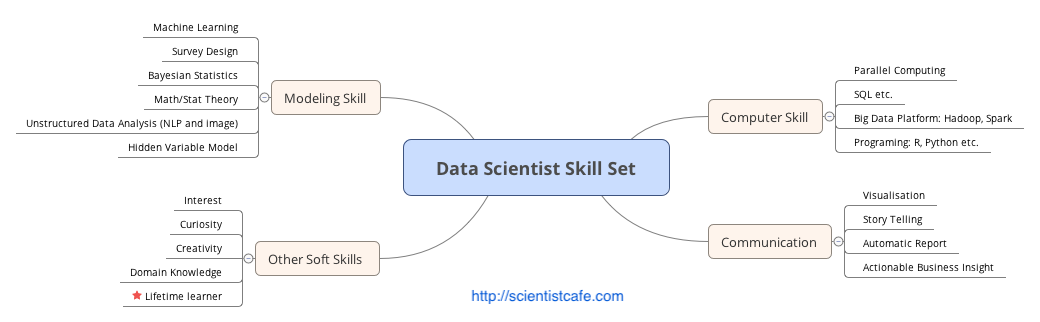
\includegraphics{images/SkillEN.png}
\caption{Data Scientist Skill Set}
\end{figure}

\section{Types of Learning}\label{types-of-learning}

There are three broad groups of styles: supervised learning,
reinforcement learning, and unsupervised learning.

In supervised learning, each observation of the predictor measurement(s)
corresponds to a response measurement. There are two flavors of
supervised learning: regression and classification. In regression, the
response is a real number such as the total net sales in 2017, or the
yield of corn next year. The goal is to approximate the response
measurement as much as possible. In classification, the response is a
class label, such as dichotomous response such as yes/no. The response
can also have more than two categories, such as four segments of
customers. A supervised learning model is a function that maps some
input variables with corresponding parameters to a response y. Modeling
tuning is to adjust the value of parameters to make the mapping fit the
given response. In other words, it is to minimize the discrepancy
between given response and the model output. When the response y is a
real value, it is intuitive to define discrepancy as the squared
difference between model output and given the response. When y is
categorical, there are other ways to measure the difference, such as AUC
or information gain.

In reinforcement learning, the correct input/output pairs are not
present. The model will learn from a sequence of actions and select the
action maximizing the expected sum of the future rewards. There is a
discount factor that makes future rewards less valuable than current
rewards. Reinforcement learning is difficult for the following reasons:

\begin{enumerate}
\def\labelenumi{(\arabic{enumi})}
\item
  The rewards are not instant. If the action sequence is long, it is
  hard to know which action was wrong.
\item
  The rewards are occasional. Each reward does not supply much
  information, so its impact of parameter change is limited. Typically,
  it is not likely to learn a large number of parameters using
  reinforcement learning. However, it is possible for supervised and
  unsupervised learning. The number of parameters in reinforcement
  learning usually range from dozens to maybe 1,000, but not millions.
\end{enumerate}

In unsupervised learning, there is no response variable. For a long
time, the machine learning community overlooked unsupervised learning
except for one called clustering. Moreover, many researchers thought
that clustering was the only form of unsupervised learning. One reason
is that it is hard to define the goal of unsupervised learning
explicitly. Unsupervised learning can be used to do the following:

\begin{enumerate}
\def\labelenumi{(\arabic{enumi})}
\item
  Identify a good internal representation or pattern of the input that
  is useful for subsequent supervised or reinforcement learning, such as
  finding clusters.
\item
  It is a dimension reduction tool that is to provide compact, low
  dimensional representations of the input, such as factor analysis.
\item
  Provide a reduced number of uncorrelated learned features from
  original variables, such as principal component regression.
\end{enumerate}

\begin{figure}[htbp]
\centering
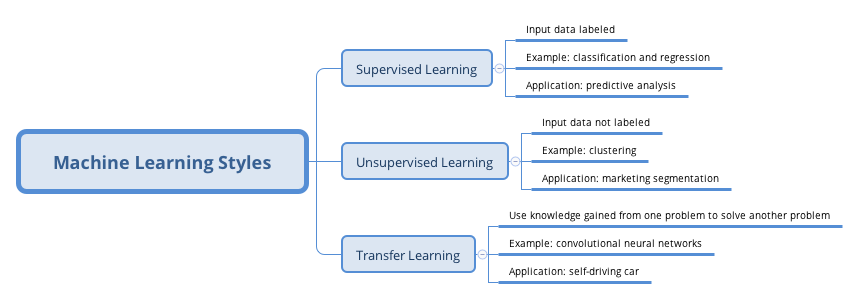
\includegraphics{images/LearningStyles.png}
\caption{Machine Learning Styles}
\end{figure}

\section{Types of Algorithm}\label{types-of-algorithm}

The categorization here is based on the structure (such as tree model,
Regularization Methods) or type of question to answer (such as
regression).\footnote{The summary of various algorithms for data science
  in this section is based on Jason Brownlee's blog ``(A Tour of Machine
  Learning
  Algorithms){[}\url{http://machinelearningmastery.com/a-tour-of-machine-learning-algorithms/}{]}.''
  We added and subtracted some algorithms in each category and gave
  additional comments.} It is far less than perfect but will help to
show a bigger map of different algorithms. Some can be legitimately
classified into multiple categories, such as support vector machine
(SVM) can be a classifier, and can also be used for regression. So you
may see other ways of grouping. Also, the following summary does not
list all the existing algorithms (there are just too many).

\begin{enumerate}
\def\labelenumi{\arabic{enumi}.}
\tightlist
\item
  Regression
\end{enumerate}

Regression can refer to the algorithm or a particular type of problem.
It is supervised learning. Regression is one of the oldest and most
widely used statistical models. It is often called the statistical
machine learning method. Standard regression models are:

\begin{itemize}
\tightlist
\item
  Ordinary Least Squares Regression
\item
  Logistic Regression
\item
  Multivariate Adaptive Regression Splines (MARS)
\item
  Locally Estimated Scatterplot Smoothing (LOESS)
\end{itemize}

The least squares regression and logistic regression are traditional
statistical models. Both of them are highly interpretable. MARS is
similar to neural networks and partial least squares (PLS) in the
respect that they all use surrogate features instead of original
predictors.

They differ in how to create the surrogate features. PLS and neural
networks use linear combinations of the original predictors as surrogate
features \footnote{To be clear on neural networks, the linear
  combinations of predictors are put through non-linear activation
  functions, deeper neural networks have many layers of non-linear
  transformation}. MARS creates two contrasted versions of a predictor
by a truncation point. And LOESS is a non-parametric model, usually only
used in visualization.

\begin{enumerate}
\def\labelenumi{\arabic{enumi}.}
\setcounter{enumi}{1}
\tightlist
\item
  Similarity-based Algorithms
\end{enumerate}

This type of model is based on a similarity measure. There are three
main steps: (1) compare the new sample with the existing ones; (2)
search for the closest sample; (3) and let the response of the nearest
sample be used as the prediction.

\begin{itemize}
\tightlist
\item
  K-Nearest Neighbour {[}KNN{]}
\item
  Learning Vector Quantization {[}LVQ{]}
\item
  Self-Organizing Map {[}SOM{]}
\end{itemize}

The biggest advantage of this type of model is that they are intuitive.
K-Nearest Neighbour is generally the most popular algorithm in this set.
The other two are less common. The key to similarity-based algorithms is
to find an appropriate distance metric for your data.

\begin{enumerate}
\def\labelenumi{\arabic{enumi}.}
\setcounter{enumi}{2}
\tightlist
\item
  Feature Selection Algorithms
\end{enumerate}

The primary purpose of feature selection is to exclude non-information
or redundant variables and also reduce dimension. Although it is
possible that all the independent variables are significant for
explaining the response. But more often, the response is only related to
a portion of the predictors. We will expand the feature selection in
detail later.

\begin{itemize}
\tightlist
\item
  Filter method
\item
  Wrapper method
\item
  Embedded method
\end{itemize}

Filter method focuses on the relationship between a single feature and a
target variable. It evaluates each feature (or an independent variable)
before modeling and selects ``important'' variables.

Wrapper method removes the variable according to particular law and
finds the feature combination that optimizes the model fitting by
evaluating a set of feature combinations. In essence, it is a searching
algorithm.

Embedding method is part of the machine learning model. Some model has
built-in variable selection function such as lasso, and decision tree.

\begin{enumerate}
\def\labelenumi{\arabic{enumi}.}
\setcounter{enumi}{3}
\tightlist
\item
  Regularization Method
\end{enumerate}

This method itself is not a complete model, but rather an add-on to
other models (such as regression models). It appends a penalty function
on the criteria used by the original model to estimate the variables
(such as likelihood function or the sum of squared error). In this way,
it penalizes model complexity and contracts the model parameters. That
is why people call them ``shrinkage method.'' This approach is
advantageous in practice.

\begin{itemize}
\tightlist
\item
  Ridge Regression
\item
  Least Absolute Shrinkage and Selection Operator (LASSO)
\item
  Elastic Net
\end{itemize}

\begin{enumerate}
\def\labelenumi{\arabic{enumi}.}
\setcounter{enumi}{4}
\tightlist
\item
  Decision Tree
\end{enumerate}

Decision trees are no doubt one of the most popular machine learning
algorithms. Thanks to all kinds of software, implementation is a
no-brainer which requires nearly zero understanding of the mechanism.
The followings are some of the common trees:

\begin{itemize}
\tightlist
\item
  Classification and Regression Tree (CART)
\item
  Iterative Dichotomiser 3 (ID3)
\item
  C4.5
\item
  Random Forest
\item
  Gradient Boosting Machines (GBM)
\end{itemize}

\begin{enumerate}
\def\labelenumi{\arabic{enumi}.}
\setcounter{enumi}{5}
\tightlist
\item
  Bayesian Models
\end{enumerate}

People usually confuse Bayes theorem with Bayesian models. Bayes theorem
is an implication of probability theory which gives Bayesian data
analysis its name.

\[Pr(\theta|y)=\frac{Pr(y|\theta)Pr(\theta)}{Pr(y)}\]

The actual Bayesian model is not identical to Bayes theorem. Given a
likelihood, parameters to estimate, and a prior for each parameter, a
Bayesian model treats the estimates as a purely logical consequence of
those assumptions. The resulting estimates are the posterior
distribution which is the relative plausibility of different parameter
values, conditional on the observations. The Bayesian model here is not
strictly in the sense of Bayesian but rather model using Bayes theorem.

\begin{itemize}
\tightlist
\item
  Naïve Bayes
\item
  Averaged One-Dependence Estimators (AODE)
\item
  Bayesian Belief Network (BBN)
\end{itemize}

\begin{enumerate}
\def\labelenumi{\arabic{enumi}.}
\setcounter{enumi}{6}
\tightlist
\item
  Kernel Methods
\end{enumerate}

The most common kernel method is the support vector machine (SVM). This
type of algorithm maps the input data to a higher order vector space
where classification or regression problems are easier to solve.

\begin{itemize}
\tightlist
\item
  Support Vector Machine (SVM)
\item
  Radial Basis Function (RBF)
\item
  Linear Discriminate Analysis (LDA)
\end{itemize}

\begin{enumerate}
\def\labelenumi{\arabic{enumi}.}
\setcounter{enumi}{7}
\tightlist
\item
  Clustering Methods
\end{enumerate}

Like regression, when people mention clustering, sometimes they mean a
class of problems, sometimes a class of algorithms. The clustering
algorithm usually clusters similar samples to categories in a centroidal
or hierarchical manner. The two are the most common clustering methods:

\begin{itemize}
\tightlist
\item
  K-Means
\item
  Hierarchical Clustering
\end{itemize}

\begin{enumerate}
\def\labelenumi{\arabic{enumi}.}
\setcounter{enumi}{8}
\tightlist
\item
  Association Rule
\end{enumerate}

The basic idea of an association rule is: when events occur together
more often than one would expect from their rates of occurrence, such
co-occurrence is an interesting pattern. The most used algorithms are:

\begin{itemize}
\tightlist
\item
  Apriori algorithm
\item
  Eclat algorithm
\end{itemize}

\begin{enumerate}
\def\labelenumi{\arabic{enumi}.}
\setcounter{enumi}{9}
\tightlist
\item
  Artificial Neural Network
\end{enumerate}

The term neural network has evolved to encompass a repertoire of models
and learning methods. There has been lots of hype around the model
family making them seem magical and mysterious. A neural network is a
two-stage regression or classification model. The basic idea is that it
uses linear combinations of the original predictors as surrogate
features, and then the new features are put through non-linear
activation functions to get hidden units in the 2nd stage. When there
are multiple hidden layers, it is called deep learning, another over
hyped term. Among varieties of neural network models, the most widely
used ``vanilla'' net is the single hidden layer back-propagation
network.

\begin{itemize}
\tightlist
\item
  Perceptron Neural Network
\item
  Back Propagation
\item
  Hopield Network
\item
  Self-Organizing Map (SOM)
\item
  Learning Vector Quantization (LVQ)
\end{itemize}

\begin{enumerate}
\def\labelenumi{\arabic{enumi}.}
\setcounter{enumi}{10}
\tightlist
\item
  Deep Learning
\end{enumerate}

The name is a little misleading. As mentioned before, it is multilayer
neural network. It is hyped tremendously especially after AlphaGO
defeated Li Shishi at the board game Go. We don't have too much
experience with the application of deep learning and are not in the
right position to talk more about it. Here are some of the common
algorithms:

\begin{itemize}
\tightlist
\item
  Restricted Boltzmann Machine (RBN)
\item
  Deep Belief Networks (DBN)
\item
  Convolutional Network
\item
  Stacked Autoencoders
\item
  Long short-term memory (LSTM)
\end{itemize}

\begin{enumerate}
\def\labelenumi{\arabic{enumi}.}
\setcounter{enumi}{11}
\tightlist
\item
  Dimensionality Reduction
\end{enumerate}

Its purpose is to construct new features that have significant physical
or statistical characteristics, such as capturing as much of the
variance as possible.

\begin{itemize}
\tightlist
\item
  Principle Component Analysis (PCA)
\item
  Partial Least Square Regression (PLS)
\item
  Multi-Dimensional Scaling (MDS)
\item
  Exploratory Factor Analysis (EFA)
\end{itemize}

PCA attempts to find uncorrelated linear combinations of original
variables that can explain the variance to the greatest extent possible.
EFA also tries to explain as much variance as possible in a lower
dimension. MDS maps the observed similarity to a low dimension, such as
a two-dimensional plane. Instead of extracting underlying components or
latent factors, MDS attempts to find a lower-dimensional map that best
preserves all the observed similarities between items. So it needs to
define a similarity measure as in clustering methods.

\begin{enumerate}
\def\labelenumi{\arabic{enumi}.}
\setcounter{enumi}{12}
\tightlist
\item
  Ensemble Methods
\end{enumerate}

Ensemble method made its debut in the 1990s. The idea is to build a
prediction model by combining the strengths of a collection of simpler
base models. Bagging, originally proposed by Leo Breiman, is one of the
earliest ensemble methods. After that, people developed Random Forest
\citep{Ho1998, amit1997} and Boosting method
\citep{Valiant1984, KV1989}. This is a class of powerful and effective
algorithms.

\begin{itemize}
\tightlist
\item
  Bootstrapped Aggregation (Bagging)
\item
  Random Forest
\item
  Gradient Boosting Machine (GBM)
\end{itemize}

\begin{figure}[htbp]
\centering
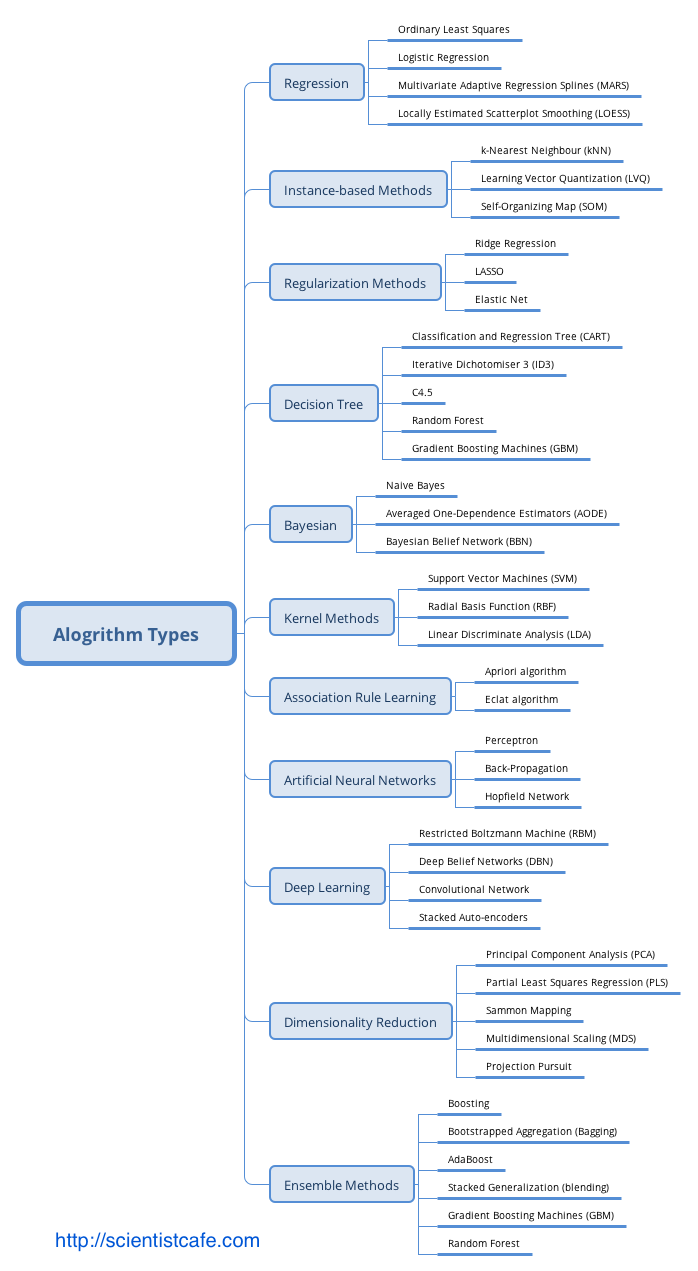
\includegraphics{images/AlogrithmTypes.png}
\caption{Machines Learning Algorithms}
\end{figure}

\chapter{Soft Skills for Data
Scientists}\label{soft-skills-for-data-scientists}

\section{Comparison between Statistician and Data
Scientist}\label{comparison-between-statistician-and-data-scientist}

Statistics as a scientific area can be traced back to 1749 and
statistician as a career has been around for hundreds of years with
well-established theory and application. Data Scientist becomes an
attractive career for only a few years along with the fact that data
size and variety beyond the traditional statistician's toolbox and the
fast-growing of computation power. Statistician and data scientist have
a lot of common backgrounds, but there are also some significant
differences.

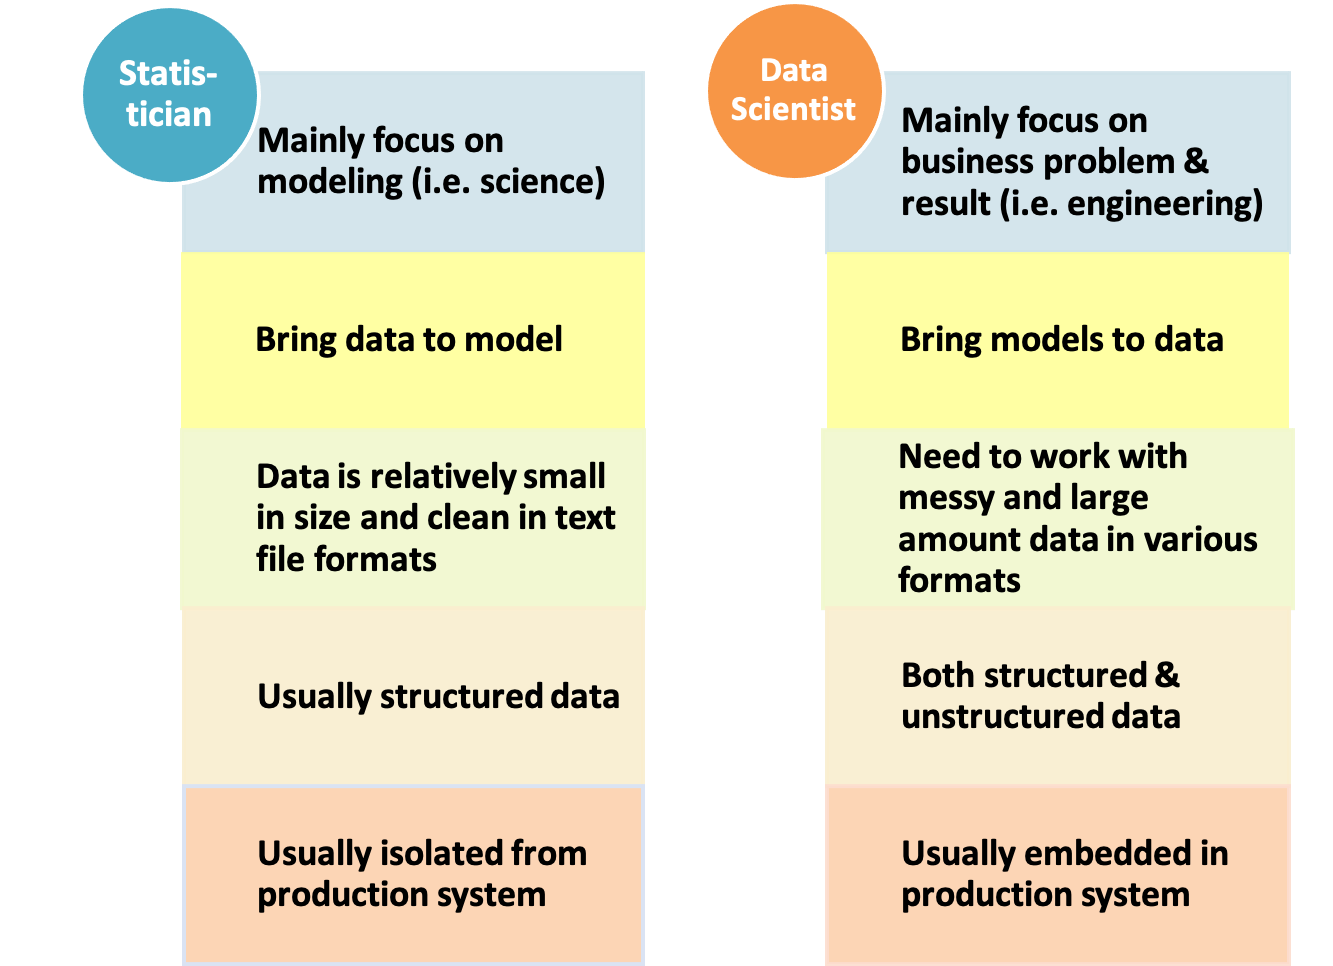
\includegraphics{images/softskill1.png}

Both statistician and data scientist work closely with data. For the
traditional statistician, the data is usually well-formatted text files
with numbers and labels. The size of the data usually can be fitted in a
PC's memory. Comparing to statisticians, data scientists need to deal
with more varieties of data: well-formatted data stored in a database
system with size much larger than a PC's memory or hard-disk; huge
amount of verbatim text, voice, image, and video; real-time streaming
data and other types of records. One particular power of statistics is
that statistician can fit model and make an inference based on limited
data. It is quite common that once the data is given and cleaned, the
majority of the work is developed different models around the data.
Today, data is relatively abundant, and modeling is just part of the
overall effort. The focus is to deliver actionable results. Different
from statisticians, data scientists, sometimes need to fit model on the
cloud instead of reading data in since the data size is too large. From
the entire problem-solving cycle, statisticians are usually not well
integrated with the production system where data is obtained in real
time; while data scientists are more embedded in the production system
and closer to the data generation procedures.

\section{Where Data Science Team
Fits?}\label{where-data-science-team-fits}

During the past decade, a huge amount of data has become available and
readily accessible for analysis in many companies across different
business sectors. The size, complexity, and speed of increment of data
suddenly beyond the traditional scope of statistical analysis or BI
reporting as mentioned above. To leverage the big data, many companies
have established new data science organizations. Companies have gone
through different paths to create their data science and machine
learning organizations. There are three major formats of data science
teams:

\begin{enumerate}
\def\labelenumi{(\arabic{enumi})}
\tightlist
\item
  independent of any current organizations and the team report directly
  to senior leadership;\\
\item
  within each business unit and the team report to business unit
  leaders;\\
\item
  within in the traditional IT organizations and the team report to IT
  leaders.
\end{enumerate}

Companies are different in many aspects, but in general, the most
efficient option to mine big data is a team of data scientist
independent of business units and IT organizations. The independence
enables the data science team to collaborate across business units and
IT organizations more efficiently and the independence also provides
flexibility and potential to solve corporate level strategic big data
problems. For each business units, there are many business unit specific
data science related problems and embedding data scientist within each
business units is also an efficient way to solve business unit specific
data science problems. The full cycle of data science projects from data
to decision (i.e.~Data -\textgreater{} Information -\textgreater{}
Knowledge -\textgreater{} Insight -\textgreater{} Decision) is
relatively difficult to achieve if the data science team is part of
traditional IT organizations.

\section{Beyond Data and Analytics}\label{beyond-data-and-analytics}

Data scientists usually have a good sense of data and analytics, but
data scientist project is more than just data and analytics. A data
science project may involve people with many different roles:

\begin{itemize}
\tightlist
\item
  a business owner or leader to identify opportunities in business
  value; program managers to ensure each data science project fit into
  the overall technical program development;
\item
  data owners and computation resource and infrastructure owners from IT
  department;
\item
  dedicated team to make sure the data and model are under model
  governance and privacy guidelines;
\item
  a team to implement, maintain and refresh the model;
\item
  project managers to coordinate all parties to set periodical tasks so
  that the project meets the preset milestones and delivery results;
\item
  multiple rounds of discussion of resource allocation (i.e.~who will
  pay for the data science project).
\end{itemize}

Effective communication and in-depth domain knowledge about the business
problem are essential requirements for a successful data scientist. A
data scientist will interact with people at various levels ranging from
senior leaders who are setting the corporate strategies to front-line
employees who are doing the daily work. A data scientist needs to have
the capability to view the problem from 10,000 feet above ground, as
well as down to the detail to the very bottom. To convert a business
question into a data problem, a data scientist needs to communicate
using the language the other people can understand and obtain the
required information.

\section{Data Scientist as a Leader}\label{data-scientist-as-a-leader}

During the entire process of data science project defining, planning,
executing and implementation, the data scientist lead needs to be
involved in every step to ensure the business problem is defined
correctly and the business value and success metric are evaluated
reasonably. Corporates are investing heavily in data science and machine
learning with a very high expectation of big return. There are too many
opportunities to introduce unrealistic goal and business impact for a
particular data science project. The leading data scientist need to be
the leader in these discussions to define the goal backed by data and
analytics. Many data science projects over promise in deliverables and
too optimistic on the timeline and these projects eventually fail by not
delivering the preset business impact within the timeline. As the data
scientist in the team, we need to identify these issues early in the
stage and communicate to the entire team to make sure the project has a
realistic deliverable and timeline. The data scientist team also need to
work closely with data owners to identify relevant internal and external
data source and evaluate the quality of the data; as well as working
closely with the computation infrastructure team to understand the
computation resources (i.e.~hardware and software) available for the
data science project.

\section{Three Pillars of Knowledge}\label{three-pillars-of-knowledge}

The following picture summarizes the needed three pillars of knowledge
to be a successful data scientist.

\begin{enumerate}
\def\labelenumi{(\arabic{enumi})}
\item
  A successful data scientist needs to have a strong technical
  background in data mining, statistics and machine learning. The
  in-depth understanding of modeling with the insight about data enable
  a data scientist to convert a business problem to a data science
  problem.
\item
  A successful data scientist needs some domain knowledge to understand
  business problem. For any data science project, the data scientist
  need to collaborate with other team members and effective
  communication and leadership skills are critical, especially when you
  are the only data person in the room and you need to decide with
  uncertainty.
\item
  The last pillar is about computation environment and model
  implementation in big data platform. This used to be the most
  difficult one for a data scientist with statistics background
  (i.e.~lack computer science or programming skills). The good news is
  that with the rise of cloud computation big data platform, this
  barrier is getting easier for a statistician to overcome and we will
  discuss in more detail in next chapter.
\end{enumerate}

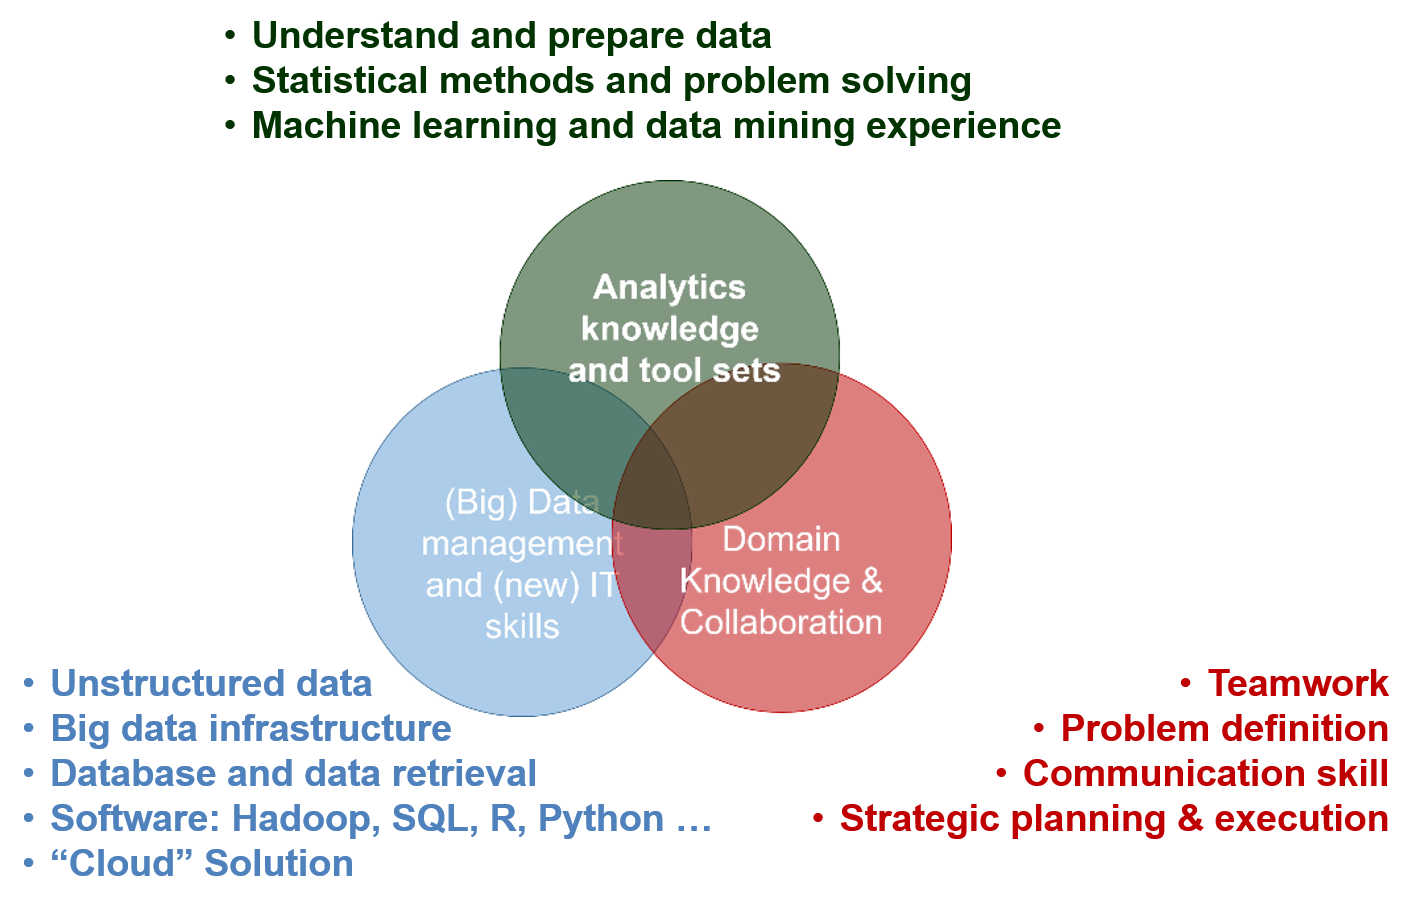
\includegraphics{images/softskill2.png}

\section{Common Pitfalls of Data Science
Projects}\label{common-pitfalls-of-data-science-projects}

Data science projects are usually complicated, and many of these data
science projects eventually fail due to various reasons. We will briefly
discuss a few common pitfalls in data science projects and how to avoid
them.

\begin{itemize}
\item
  \textbf{Solve the wrong problem:} data science project usually starts
  with a very vague description and a few rounds of detailed discussion
  with all stakeholders involved are needed to define the busses
  problem. There will be lots of opportunities to introduce misalignment
  when mapping the business problem into specific data science methods.
  Especially when the quality and availability of the data are not as
  good as what is expected at the first place. If not well-communicated
  during the project, the final data science solution may not be the
  right one to solve the business problem. As the data scientist
  (sometimes the only data scientist) in the room, we must understand
  the business problem thoroughly and communicate regularly to business
  partners especially there is a change of status to make sure everyone
  is aligned with the progress and final deliverables.
\item
  \textbf{Over promise on business value:} business leaders usually have
  high expectation on data science projects and the goal of business
  value and deliverables sometimes are set unrealistic and eventually
  beyond the scope of available data and computation resource. As the
  data scientist (sometimes the only data scientist) in the room, we
  must have our voice heard based on fact (i.e.~data, analytics, and
  resources) instead of wishful thinking. Backed with fact-based
  evidence, it is easier to communicate what is a realistic goal for the
  entire team.
\item
  \textbf{Too optimistic about the timeline:} there are lots of
  uncertainties in data science projects such as the data source
  availability and data quality, computation hardware and software,
  resource availability in the business team, implementation team and IT
  department, as well as project direction change which may delay the
  final delivery date. To have a better-estimated timeline, get as much
  detail as possible for all the needed tasks and estimated each task
  individually and reach out to each team member to confirm their
  availability. Most importantly, communicate with the entire team if
  there are blocking factors for the project in a prompt way such that
  everyone aware of the situation and potential impact on the timeline.
\item
  \textbf{Too optimistic about data availability and quality:} the most
  important asset in data science project is data. Even though we are at
  the big data age, often there is not enough relevant data for the data
  science projects. The data quality is also a general problem for data
  science projects. A thorough data availability and quality check are
  needed at the beginning of the data science project to estimate the
  needed effort to obtain data as well as data cleaning.
\item
  \textbf{Model cannot be scaled:} be careful if you use a subset of
  data to fit the model and then scale it to the entire dataset. When
  developing the model using a smaller dataset, we must keep in mind how
  much computation resources needed for the whole dataset. With limited
  computation resource, it is important to maximize the computation time
  in production to a reasonable level based on the business application
  when fits the model with a sample dataset.
\item
  \textbf{Take too long to fail:} data science projects usually are
  trying to push the boundary of current applications to new territory,
  people do not expect all data science projects to be successful. Fail
  fast is good practice such that we can quickly find a better way to
  solve the problem. A data scientist needs to have an open mindset to
  not stuck with one idea or one approach for a long time to avoid
  taking too long to fail.
\end{itemize}

\chapter{References}\label{references}

\bibliography{bibliography.bib}

\backmatter
\printindex

\end{document}
